\vspace*{1.5pc}


\subsection{Cosmological Parameters}

\begin{figure}
\begin{center}
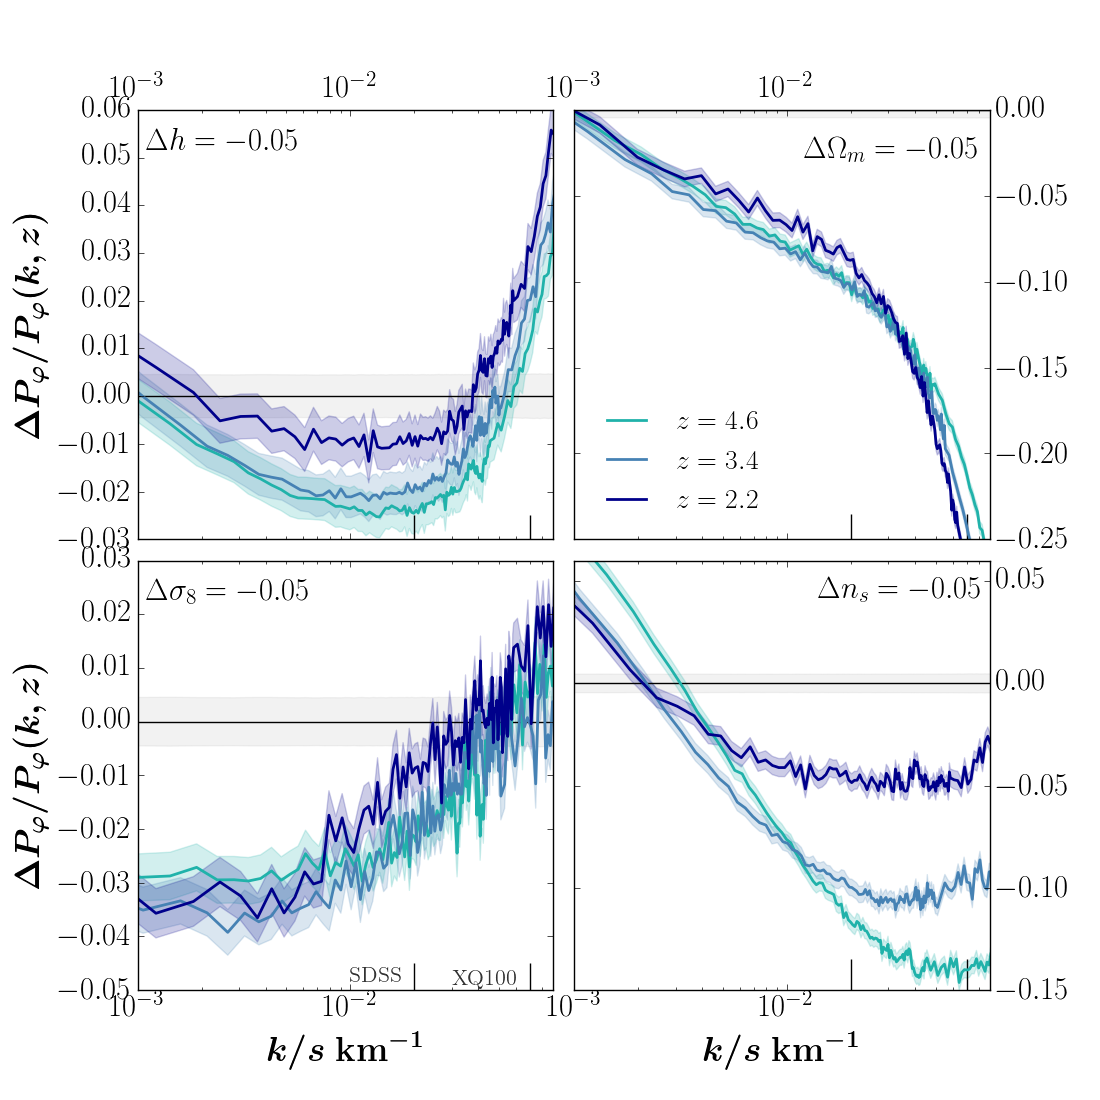
\includegraphics[width = 16cm]{Cosmo_Pf.png}
\caption{Relative difference in flux power spectrum with respect to the central \textit{best guess} model (black line) which is set at $\vec{x}_0^{\mathrm{cosmo}} = \left( h = 0.675, \Omega_m = 0.31, n_s = 0.96, \sigma_8 = 0.83 \right)^T$. Clockwise from top left panel: $\Delta x_i = -0.05$ value on $h, \Omega_m, n_s$ and $\sigma_8$ (\textit{i.e.} lower step value in Tab.~\ref{tab:parameter_values}). Statistical uncertainty on $P_\varphi (k)$ is encoded in the shade thickness. The redshift dependance is featured in the dark blue, light blue and teal curves which correspond to $z=2.2, 3.4$ and $4.6$ respectively. The `SDSS' and `XQ100' ticks refer to the highest data $k$ mode in each survey.}
\label{fig:Cosmo_flux}
\end{center}
\end{figure}


In this section, I issue the most up-to-date results on cosmological parameters constrained with the Ly-$\alpha$ forest power spectrum in the context of a benchmark $\Lambda$CDM model. Fig.~\ref{fig:Cosmo_flux} shows the computed flux power spectra of $h=0.625$, $\Omega_m=0.26$, $n_s=0.91$ and $\sigma_8=0.78$ in three distinct redshifts, normalised to the \emph{best guess} values of $h=0.675$, $\Omega_m=0.31$, $n_s=0.96$ and $\sigma_8=0.83$. Each power spectrum is normalised to its corresponding value of $\sigma_8$ at each redshift. The best-fitted values in our analysis described in Sec.~\ref{sec:methodology} along with their $68\%$ C.L.  are grouped in Tab.~\ref{tab:best_fit}, when using the Ly-$\alpha$ power spectrum in addition to an expansion rate value of $H_0 = 67.3 \pm 1.0 \; \rm{km~s^{-1}~Mpc^{-1}}$ (Ly-$\alpha$ + $H_0$, see Sec.~\ref{sec:data}). The left-hand column uses the flux power spectrum from BOSS DR9, which covers velocity-space modes up to $k \sim 2 \times 10^{-2}~s/\mathrm{km}$. The right-hand column features our fitted parameters when using both the BOSS DR9 flux power spectrum with that of the XQ-100 sample in 3 redshift bins, which cover scales down to $k \sim 7 \times 10^{-2}~s/\mathrm{km}$. All cosmological parameters with the exception of the spectral index are consistent with the values obtained by the Planck collaboration on the temperature auto-correlation power spectrum on the cosmic microwave background. \\


\begin{table}
\begin{center}
\begin{tabular}{lcc}
\hline \\[-10pt]
\textbf{parameter} & \multicolumn{2}{c}{\textbf{Ly-$\alpha$ + $H_0$}} \\[2pt]
 & \textbf{SDSS/BOSS DR9} & \textbf{SDSS + XQ-100}\\[2pt]
\hline \\[-10pt]
\\ [2pt]
$h$ & $0.673 \pm 0.010$ & $0.671 \pm 0.010$ \\[2pt]
$\Omega_m$ & $0.293 \pm 0.014$ & $0.279 \pm 0.011$ \\[2pt]
$\sigma_8$ & $0.831 \pm 0.031$ & $0.797 \pm 0.023$ \\[2pt]
$n_s$ & $0.939 \pm 0.010$ & $0.956 \pm 0.007$ \\[2pt]
%\hline \\[-10pt]
%$d n_s / d \ln k$ & . & . \\[2pt]
%$N_{\mathrm{eff}}$ & . & . \\[2pt]
\hline \\[-10pt]
%$z_\star$ & . & . \\[2pt]
$T_0^{z=3}/10^3\mathrm{K}$ & $8.9^{+3.8}_{-4.0}$ & $12.8 \pm 3.1$ \\[2pt]
$\eta^{T_0}_{z<3}$ & $-2.9 \pm 0.5$ & $-2.0 \pm 0.5$ \\[2pt]
$\eta^{T_0}_{z>3}$ & $-4.4 \pm 1.1$ & $-2.2 \pm 0.8$ \\[2pt]
$\gamma^{z=3}$ & $0.9 \pm 0.1$ & $0.9 \pm 0.2$ \\[2pt]
$\eta^{\gamma}$ & $0.8 \pm 0.5$ & $-0.3 \pm 0.5$ \\[2pt]
$A^{\tau}/10^{-3}$ & $2.5 \pm 0.1$ & $3.0 \pm 0.1$ \\[2pt]
$\eta^{\tau}$ & $3.73 \pm 0.02$ & $3.66 \pm 0.01$ \\[2pt]
$f_{\mathrm{Si}\textsc{iii}}/10^{-3}$ & $5.9 \pm 0.4$ & $5.5 \pm 0.4$ \\[2pt]
$f_{\mathrm{Si}\textsc{ii}}/10^{-3}$ & $0.7 \pm 0.5$ & $0.7 \pm 0.4$ \\[2pt]
%\hline \\[-10pt]
%\textbf{reduced $\chi^2$} & $0.99$ & . \\[2pt]
\hline \\[-10pt]
\end{tabular}
\end{center}
\caption{Best fitted values and their $68\%$ C.L. of all our parameters using Ly-$\alpha$ + $H_0$ data only (BOSS alone and BOSS+XQ-100)}
\label{tab:best_fit}
\end{table}


\subsection{Running on the Spectral Index}

Our best-fit value on the spectral index is $n_s \simeq 0.939 \pm 0.010$, which we measure at $k \simeq 0.7~\mathrm{Mpc}^{-1}$ with the Ly-$\alpha$ forest. This value is at a $2\sigma$ tension with the value obtained from Planck, $n_s \simeq 0.97$ measured at $k = 0.05~\mathrm{Mpc}^{-1}$, which is arguably significant. This tension could be the result of a yet unaccounted-for systematic in our approach. It could also be a $\sim 3 \sigma$ detection of non-zero running on the spectral index, $d n_s / d \ln k > 0$, see Eq.~\ref{eq:PS_nrun}. \\

We can estimate the value of  $d n_s/d \ln k$  from the difference of scale factors at the CMB and Ly$\alpha$ pivot scales listed in the previous paragraph. Given the definition of running of Eq.~\ref{eq:PS_nrun}, and the values of $n_s$ determined separately from CMB and Ly$\alpha$ data, we estimate $d n_s/d \ln k$ to be approximately $-0.02$. This is in  agreement with the best-fit value $ -0.0178_{-0.0048}^{+0.0054} $, thus confirming that running is indeed detected in this work mostly from the different levels of $n_s$ in CMB and Ly$\alpha$ data, and thus mostly from a first order measurement of the Ly$\alpha$ power spectrum.  Any unidentified systematic uncertainty that would resolve the tension on $n_s$ would thus simultaneously annihilate our detection of $d n_s/d \ln k$. \\

\begin{figure}
\begin{center}
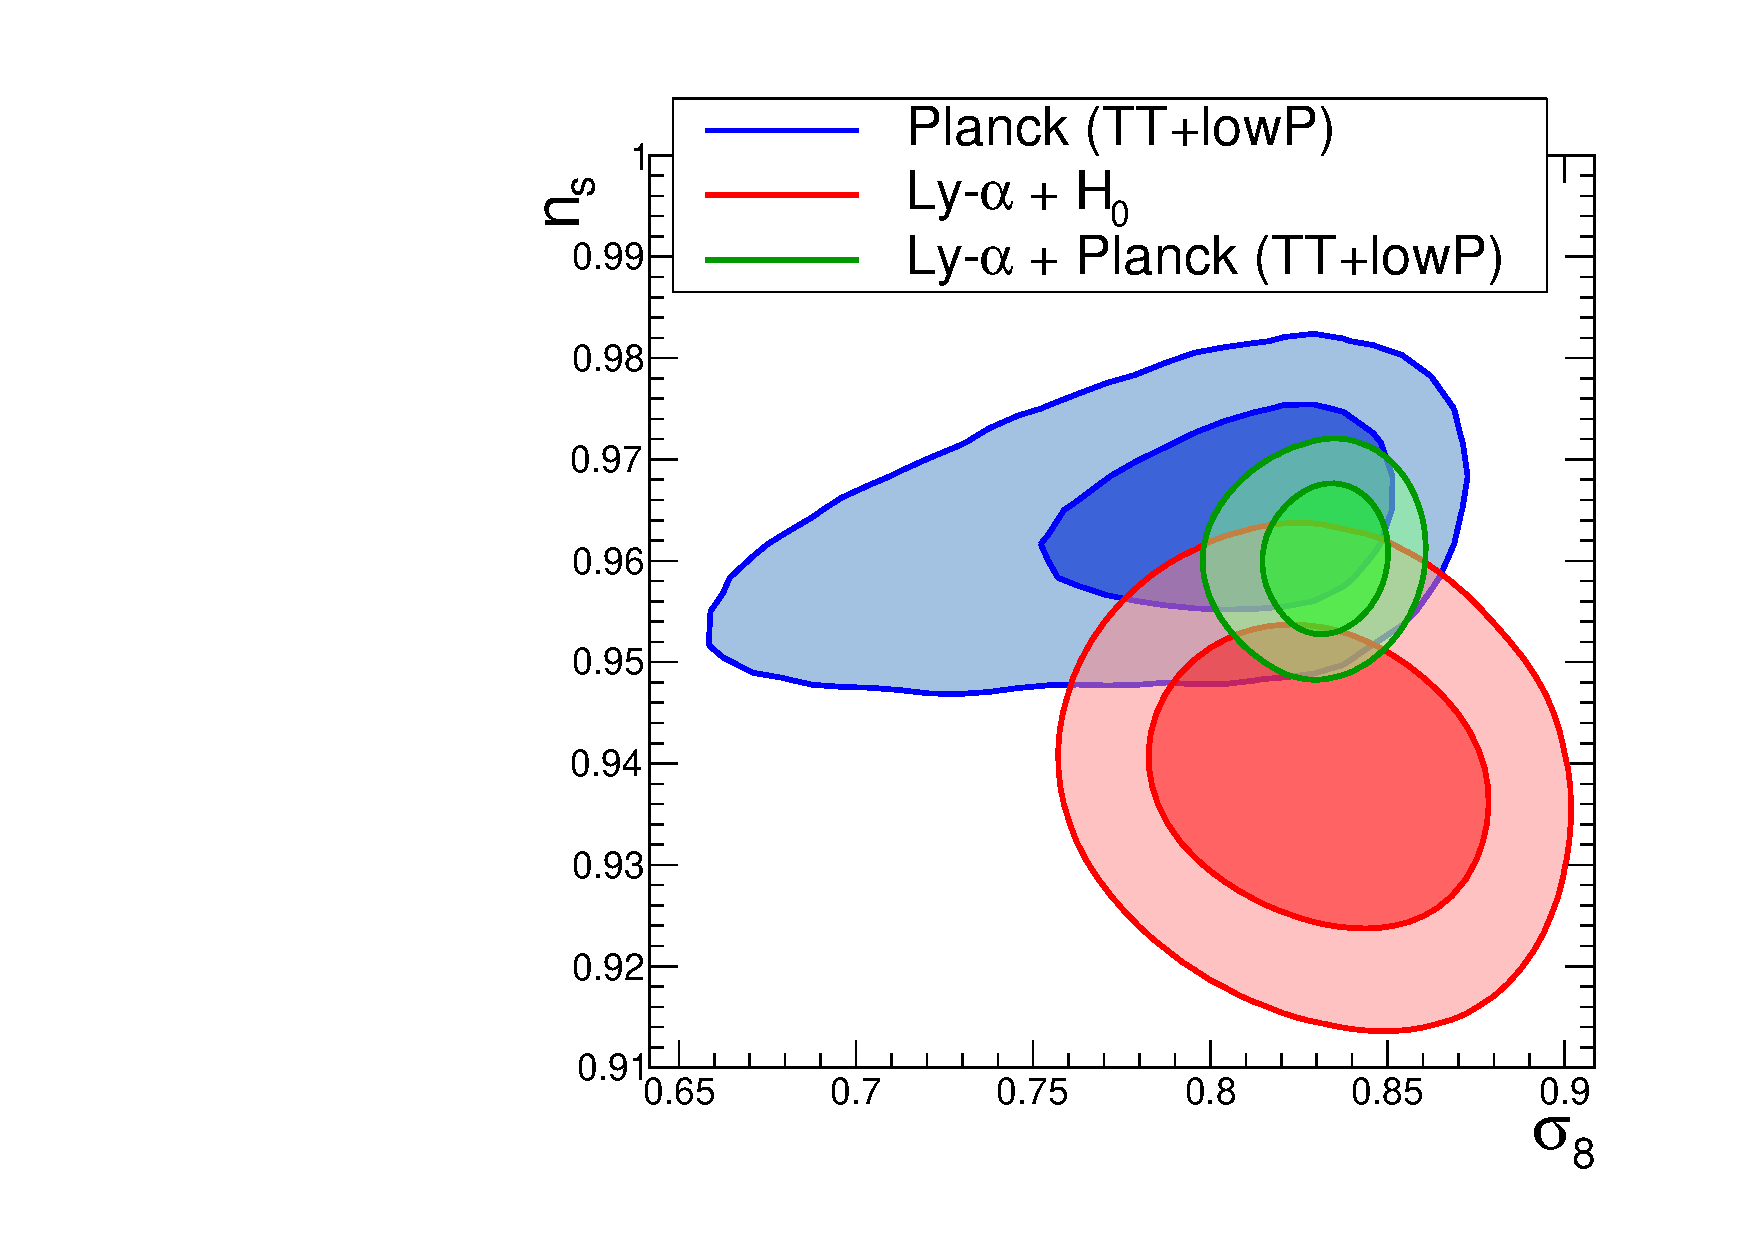
\includegraphics[width=0.55\columnwidth]{Mnu/sigma8nsLyaPlanck2015.pdf}~%
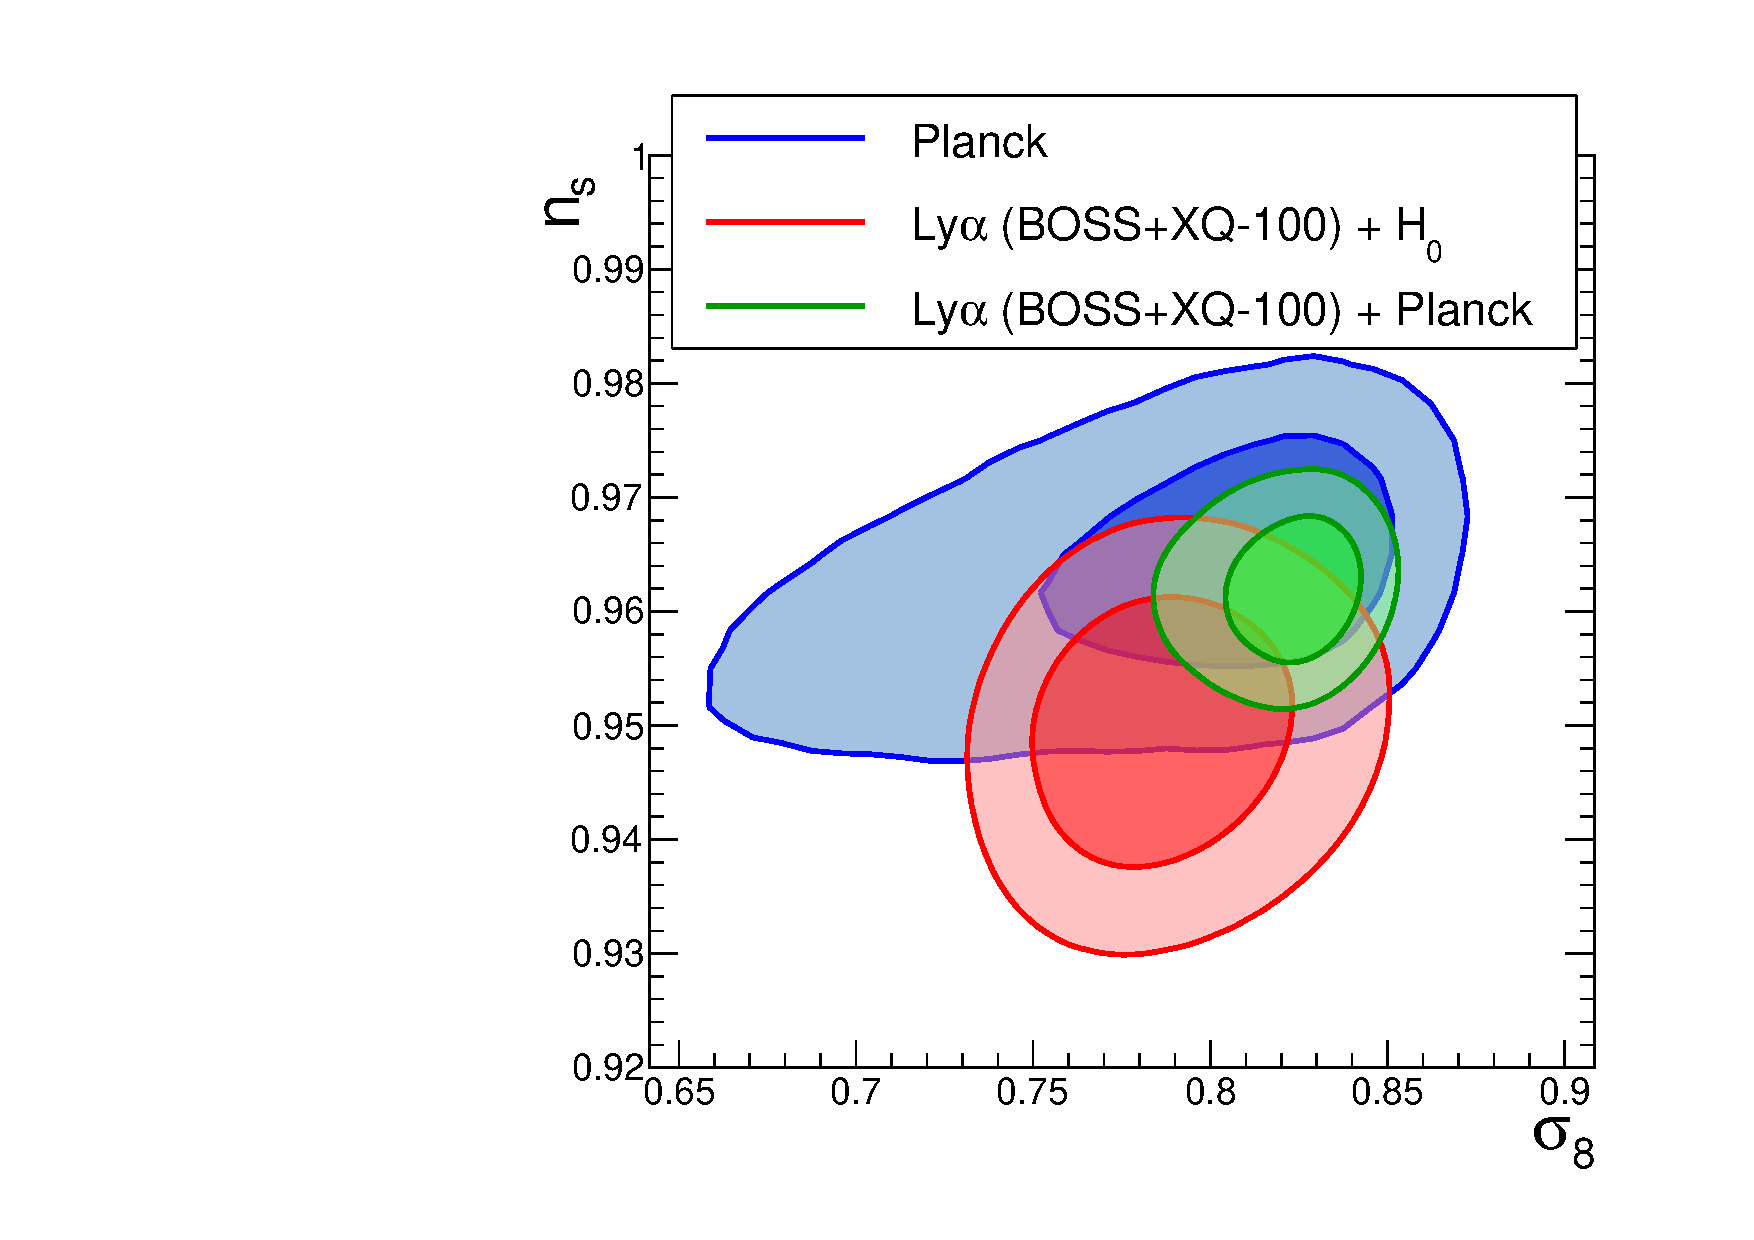
\includegraphics[width=0.55\columnwidth]{Mnu/sigma8_ns_Planck_Lya.pdf}
\caption{$68\%$ and $95\%$ C.L. in $\left( n_s, \sigma_8 \right)$ using different data sets.}
\label{fig:c2d_ns}
\end{center}
\end{figure}

Ly-$\alpha$ and CMB data being relevant on different scales, I will distinguish two cases in the upcoming sections on non cold dark matter when combining Ly-$\alpha$ data with CMB; the first fixing the running on the spectral index to its best fitted value; the other letting the running be a free parameter in the likelihood analysis. The latter reconciles the different values of $n_s$ measured at small (with Ly-$\alpha$) and large (with CMB) scales. The small discrepancy on $n_s$ between Ly-$\alpha$ and CMB measurements, and the subsequent detection of $n_{\rm run}$ at  $\sim3\sigma$, were extensively discussed in~\cite{Palanque2015b}. This ``free running'' configuration, however, is to be considered with caution. The detection of running is driven by the different values of $n_s$ measured on large and small scales. As was explained in \cite{Palanque2015b},  the determination of $n_s$ in Ly-$\alpha$ data is prone to  systematic effects in the measurement of the flux power spectrum, such as modeling of the  spectrograph resolution or contributions from SN or AGN feedbacks, UV fluctuations, \textit{etc}. The measure of $n_s$ in Ly-$\alpha$ data is  a delicate task that could still be affected by an unaccounted-for systematic. \\

Although I judge this discrepancy in $n_s$ to be mentionworthy, our research has shown that allowing for running does not affect the limit on $\sum m_\nu$ obtained for the C+HDM project (see Sec.~\ref{sec:lcdmnu}), and $n_s$ shows no distinctive correlation with the mass of warm dark matter in the pure and mixed WDM projects (see Sec.~\ref{sec:pureWDM} and \ref{sec:cwdm_flux}) as I will detail shortly. Furthermore, when adding the XQ-100 data to our Ly-$\alpha$ forest power spectrum, the value we obtain on $n_s$ falls within one standard deviation of the value measured by Planck on the CMB, as is apparent in Fig.~\ref{fig:c2d_ns}.

\subsection{Astrophysical Parameters}

\begin{figure}
\begin{center}
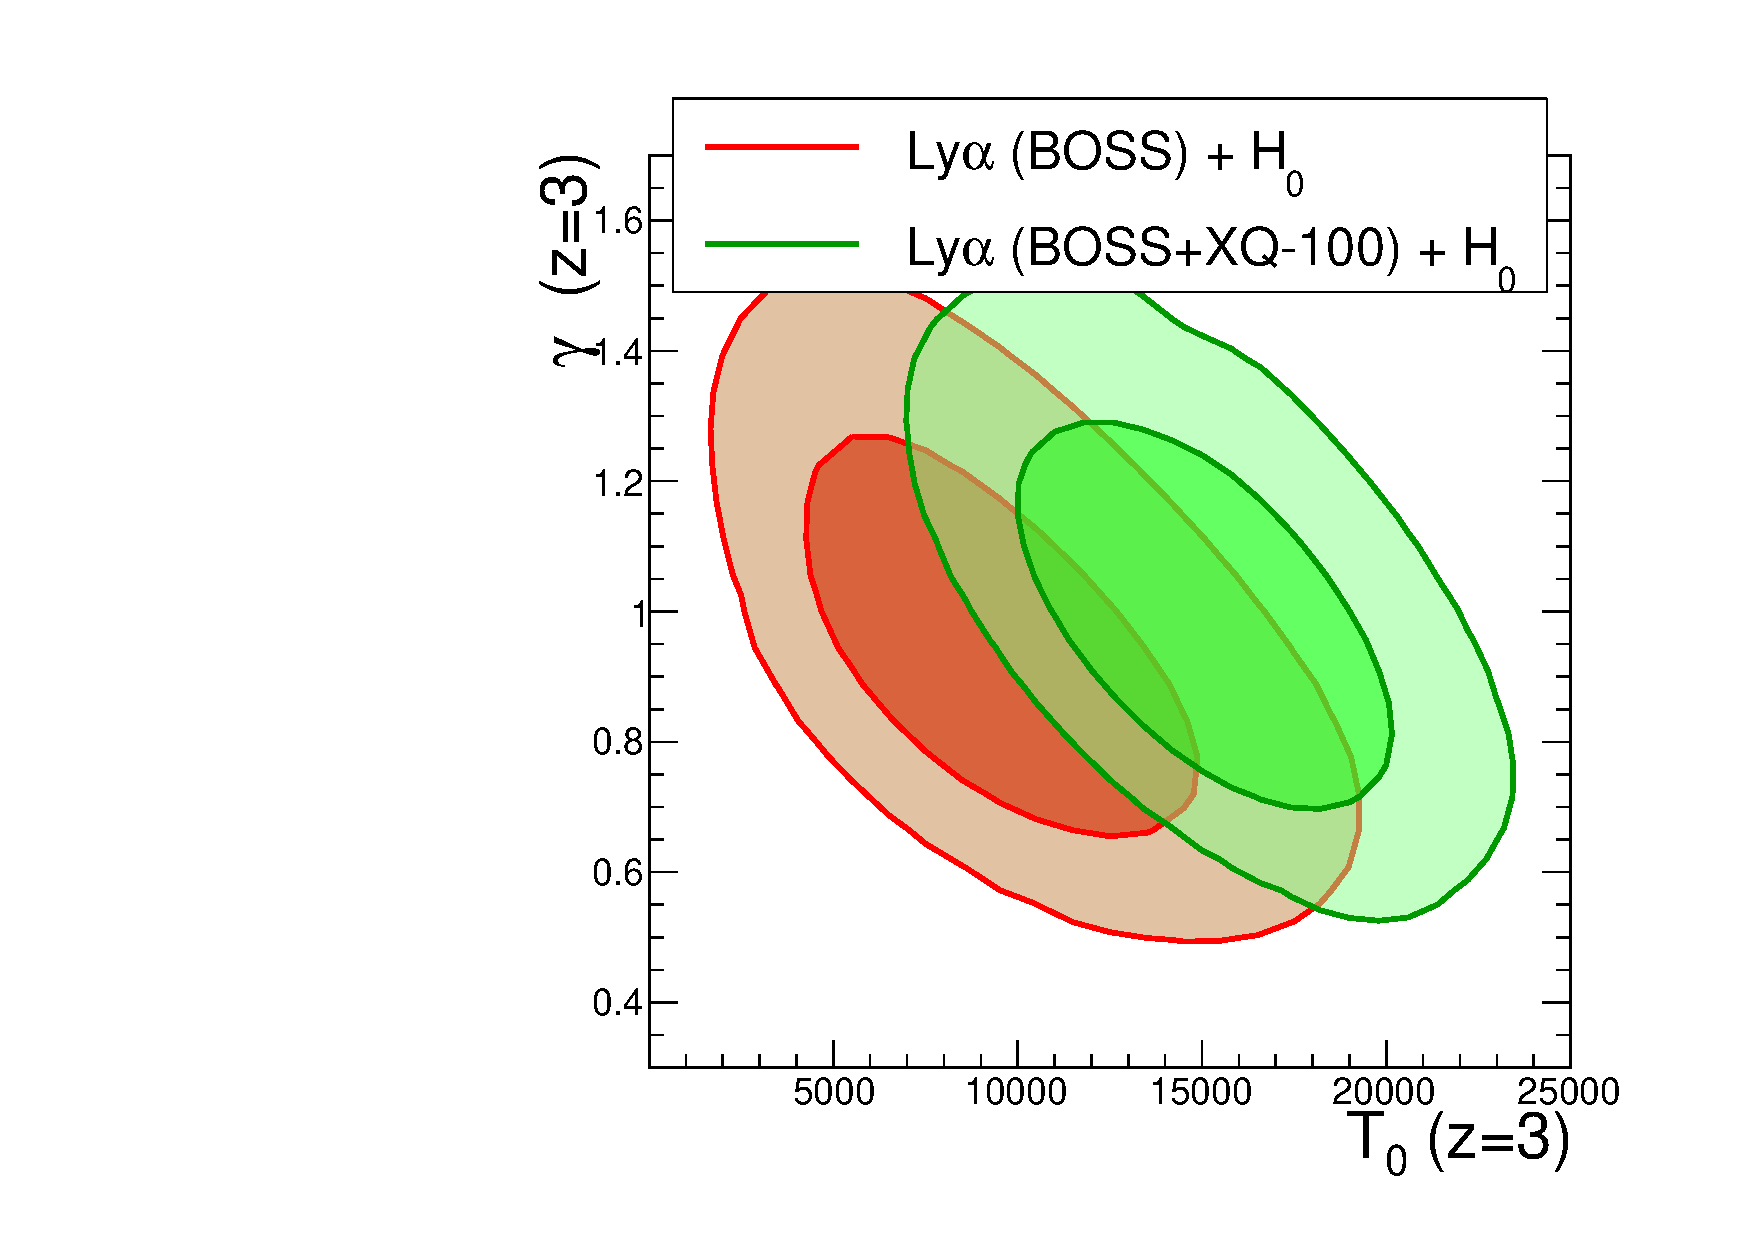
\includegraphics[width=0.75\columnwidth]{Mnu/T0_gamma.pdf}
\caption{$68\%$ and $95\%$ C.L. in the $\left( T_0^{z=3}, \gamma^{z=3} \right)$ plane using BOSS DR9 only (orange) and BOSS+XQ-100 (green) for our Ly-$\alpha$+$H_0$ data sets.}
\label{fig:c2d_igm}
\end{center}
\end{figure}

Because of a sparse data on the IGM thermal state, the values for $T_0^{z=3}$ and $\gamma^{z=3}$ in our simulation parameter grid were allowed to vary by large steps. When using higher resolution Ly-$\alpha$ data with XQ-100 in addition to BOSS, our best fitted value on the IGM background temperature (at $\delta=0$) is significantly larger ($T_0^{z=3} \simeq 1.5 \times 10^4~\mathrm{K}$) than when using BOSS only ($T_0^{z=3} \simeq 1.0 \times 10^4~\mathrm{K}$), visible in Fig.~\ref{fig:c2d_igm}. This $\sim 50\%$ discrepency suggests that the decrease in power in the Ly-$\alpha$ forest power spectrum in the right panel of Fig.~\ref{fig:data_lya} can be accounted for by a warmer IGM, as suggested in \cite{warmIGM}, and not necessarily by the free-streaming effect of a non cold dark matter particle which is expected to also cutoff power in the high-$k$ region of the power spectrum. It is visible on both panels of Fig.~\ref{fig:data_lya} that the power spectrum measured by BOSS DR9 does not probe those lower scales at which the power suppression manifests, and as such can allow for much more freedom over IGM thermal histories. 

%Caution should therefore be warranted when quoting bounds optained by BOSS DR9 data only, especially for the WDM and C+WDM and RPSN as cool dark matter investigations. It is paramount to combine with higher-resolution Ly-$\alpha$ data in those cases if the bounds on right-handed neutrinos masses $m_{\nu_s}$ are to be credible. For bounds on left-handed neutrino masses $\sum m_\nu$ in the context of the C+HDM investigation, the free-streaming effect has a distinctive cutoff profile that is not degenerate with the warm IGM Jeans scale, and so the discussion here is less relevant. 

Nevertheless, the astrophysical parameters are in good agreement when fitting with BOSS only and XQ-100 only, the largest difference being on $T_0$ at the $1.7\sigma$ level ($T_0^{z=3} = (8.9 \pm 3.9) \times 10^3~\mathrm{K}$ for BOSS only, $(21.4 \pm 6.0) \times 10^3~\mathrm{K}$ for XQ-100 only). All parameters are correlated and so it isn't straightforward to interpret this difference between the two surveys. Fig.~\ref{fig:c2d_igm} features, for instance, the strong anti-correlation between $T_0$ and $\gamma$. As a result, a low value of $\gamma$  pushes $T_0$ to high values. In the C+HDM analysis, the likelihood is built in such a way as not to be too sensitive to underlying assumptions on IGM parameters, which we here treat as nuisance parameters. The shapes of $T_0(z)$ and $\gamma(z)$ are let free in the maximization of the likelihood as explained in Sec.~\ref{sec:astro_param}.
  
\clearpage